\bookchapter{Training a kick}\label{ch:mj4}

\section*{Explanation}
A soccer robot that can walk is half of a player. The other half is a \textbf{kick}: hit a ball that lies somewhere in front of the robot so that it goes in a chosen direction with a chosen speed, and stay on the feet. A kick is a difficult motion for reinforcement learning, for four reasons: the robot stands on \emph{one leg} while the other leg swings; the contact with the ball lasts a few milliseconds, so the reward comes very late; the result depends on small details (where on the ball, with which part of the foot); and a fall is likely.

\begin{keyidea}[What exists and what does not]
In the repositories that I read (mjlab and booster-mjlab) \textbf{there is no kick task}. What exists are the pieces from which you build one: a tracking task that follows a reference motion (the T1 tracking configuration of booster-mjlab names a kicking clip from a motion-capture set as its default example, which is not distributed), AMP tasks that learn a style from clips, a get-up task, and the events and commands of mjlab. This chapter is therefore a \emph{plan}: how I would go about it, what to measure and what to check. None of it was trained; the small program of this chapter checks the physics and the reward functions, and it was run.
\end{keyidea}

\section*{What do we want from a kick?}
Write the requirement as numbers before you write any reward:
\begin{itemize}[nosep]
 \item \textbf{Direction}: the ball leaves within $\pm5^{\circ}$ of the commanded direction.
 \item \textbf{Distance}: the ball rolls the commanded distance (for example $2$\,m for a pass, $5$\,m or more for a long kick) within $\pm20\%$.
 \item \textbf{Robustness}: the robot stays upright, in $\ge95\%$ of the trials, for balls at the positions that the walking behaviour delivers.
 \item \textbf{Time}: from the start of the kick to the next ability to walk, in a few seconds. The rules of Chapter~\ref{ch:rc4}: a striker that dithers is penalised for local game stuck after $10$\,s.
 \item \textbf{Rules}: a goal cannot be scored directly from the kick-off, a robot must not push an opponent, and a free kick has to be taken within $45$\,s. These decide which \emph{variants} of the kick you need (pass, shot, clearing kick).
\end{itemize}

\section*{The physics: how fast must the foot be?}
The ball leaves with a speed that depends on the speed of the foot, on the masses and on the \textbf{restitution} (the bounciness of the contact). For a centred hit, in one dimension, a foot of effective mass $m_f$ moving at $v_f$ and a ball of mass $m_b$ at rest give the ball the speed
\[
v_b=\frac{(1+e)\,m_f}{m_f+m_b}\;v_f .
\]
After the contact the ball \textbf{rolls and slows down}. With a constant rolling deceleration $a$ it travels $d=v_b^2/(2a)$. The numbers that I use are \emph{assumptions}: $m_b=0.3$\,kg, $m_f=1.5$\,kg, $e=0.6$ and $a=0.5$\,m/s$^2$. The real values of your ball, your turf and your leg \textbf{must be measured} (see below).

\begin{center}
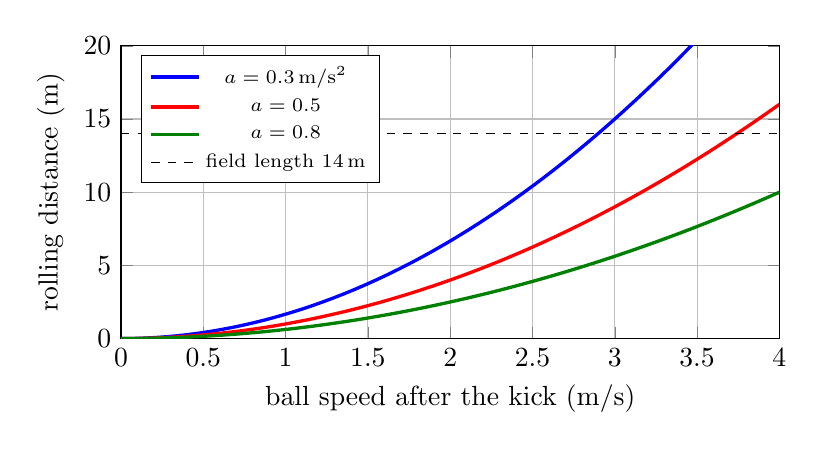
\begin{tikzpicture}
\begin{axis}[width=0.82\linewidth,height=5.3cm,xlabel={ball speed after the kick (m/s)},ylabel={rolling distance (m)},xmin=0,xmax=4,ymin=0,ymax=20,grid=both,samples=60,legend style={font=\scriptsize,at={(0.03,0.97)},anchor=north west}]
 \addplot[blue,very thick,domain=0:4] {x^2/(2*0.3)};
 \addplot[red,very thick,domain=0:4] {x^2/(2*0.5)};
 \addplot[green!50!black,very thick,domain=0:4] {x^2/(2*0.8)};
 \addplot[black,dashed,domain=0:4] {14};
 \legend{$a=0.3$\,m/s$^2$,$a=0.5$,$a=0.8$,field length $14$\,m}
\end{axis}
\end{tikzpicture}
\captionof{figure}{Rolling distance $d=v^2/(2a)$ for three values of the deceleration. The distance grows with the \emph{square} of the speed, so a small error in the speed becomes a large error in the distance: $10\%$ too fast is $21\%$ too far. A turf with a high rolling resistance (large $a$) needs a much faster kick for the same distance.}
\end{center}

\begin{example}
With the assumed values, a foot speed of $2$\,m/s gives a ball speed of $\tfrac{1.6\cdot1.5}{1.8}\cdot2=2.67$\,m/s and a rolling distance of $7.1$\,m (the program below prints this; stepping the equation of motion in time gave $7.13$\,m). A pass of $2$\,m needs a foot speed of only $1.06$\,m/s, a shot of $8$\,m $2.12$\,m/s. The feet of a walking humanoid swing at well below $1$\,m/s in normal walking. A strong kick is therefore a \emph{fast} motion that the walking policy has never seen, and that is why you cannot get it from a walking policy by changing the command.
\end{example}

\begin{verbatim}
import numpy as np

# --- Physics of one kick (all numbers are ASSUMPTIONS for illustration) ---
M_BALL, M_EFF, E = 0.30, 1.5, 0.6   # ball mass, foot mass, restitution
A_ROLL = 0.5                        # rolling deceleration (m/s^2)

def ball_speed(v_foot):
    """1-D collision of a foot of effective mass M_EFF with a ball."""
    return (1 + E) * M_EFF / (M_EFF + M_BALL) * v_foot

def roll_distance(v_ball, a=A_ROLL):
    return v_ball**2 / (2 * a)

def foot_speed_for(distance, a=A_ROLL):
    v_ball = np.sqrt(2 * a * distance)
    return v_ball * (M_EFF + M_BALL) / ((1 + E) * M_EFF)

# --- Reward terms for a kick task, written for a batch of environments ---
def r_approach(foot_pos, ball_pos, contact_done, sigma=0.3):
    """Before contact: bring the kicking foot to the ball."""
    d2 = np.sum((foot_pos - ball_pos)**2, axis=-1)
    return np.exp(-d2 / sigma**2) * (~contact_done)

def r_ball_velocity(ball_vel, cmd_vel, contact_done, sigma=0.5):
    """After contact: the ball must leave with the commanded velocity."""
    e2 = np.sum((ball_vel - cmd_vel)**2, axis=-1)
    return np.exp(-e2 / sigma**2) * contact_done

if __name__ == "__main__":
    for v in (1.0, 2.0, 3.0):
        vb = ball_speed(v)
        print(f"foot {v:.1f} -> ball {vb:.2f} m/s,",
              f"rolls {roll_distance(vb):.1f} m")
    for d in (2.0, 5.0, 8.0):
        print(f"{d:.0f} m needs {foot_speed_for(d):.2f} m/s of foot")
    cmd = np.array([[2.6, 0.0]])
    print(r_ball_velocity(np.array([[2.4, 0.0]]), cmd, np.array([True])))
    print(r_ball_velocity(np.array([[2.4, 0.5]]), cmd, np.array([True])))
    foot, ball = np.array([[0.1, 0, 0]]), np.array([[0.2, 0, 0]])
    print(r_approach(foot, ball, np.array([False])))
\end{verbatim}

\section*{Three ways to get a kick}
\textbf{A. Track a kick clip (BeyondMimic style).} Take a motion-capture clip of a kick, retarget it to the K1, convert it (Chapter~\ref{ch:mj3}) and train a tracking policy. Advantages: the most direct route; the reference solves the hard exploration problem (where is the foot supposed to go?) and gives a natural, balanced motion. Disadvantages: the direction and the strength are those of the clip; the ball is not part of the task, so the robot must be placed so that the foot meets it. To make it usable, randomise the position of the \emph{ball} and of the \emph{start pose} in the training (the ball is added as an entity of the scene) and add a reward for the ball velocity; you then have approach B with a reference.

\textbf{B. Learn the kick with a ball and a task reward.} The scene contains the ball (a free body with a sphere), the command is a \textbf{target ball velocity} (direction and speed), and the reward asks for it. This is the most flexible, but the hardest to train. With \textbf{AMP} (Chapter~\ref{ch:mj3}) a style term from walking and kicking clips keeps the motion human-like and helps against the typical solutions of a pure task reward: a bizarre hop on the support leg, a swing with the knee locked, a robot that falls on the ball.

\textbf{C. A chain of skills.} A \textbf{walking} policy (velocity tracking, Chapter~\ref{ch:mj2}) or the target-location policy of booster-mjlab brings the robot to a kick position behind the ball; then the \textbf{kick policy} is started; then walking again. The behaviour of Chapter~\ref{ch:rc2} decides when to switch. The important point is the \emph{hand-over}: the kick policy must be trained from the states in which the walking policy ends. Practical solution: record the end states of walking episodes and use them as the \emph{start distribution} of the kick training.

My recommendation for a first project is A to get a working kick quickly, and B (with AMP) once the pipeline works, to make it flexible.

\section*{Designing the kick task}
\begin{center}
\begin{tikzpicture}[>={Stealth[length=2.2mm]},ph/.style={draw,thick,minimum height=0.8cm,font=\scriptsize,align=center,anchor=west}]
 \node[ph,fill=blue!10,minimum width=2.6cm] (a) at (0,0) {approach\\ foot to ball};
 \node[ph,fill=gray!15,minimum width=1.6cm] (b) at (2.6,0) {wind-up};
 \node[ph,fill=orange!20,minimum width=1.6cm] (c) at (4.2,0) {swing};
 \node[ph,fill=red!20,minimum width=0.9cm] (d) at (5.8,0) {hit};
 \node[ph,fill=green!12,minimum width=3.2cm] (e) at (6.7,0) {follow-through,\\ recover, stand};
 \draw[<->,thick,blue!60!black] (0,-1.0)--(5.8,-1.0) node[midway,below,font=\scriptsize]{reward: foot close to the ball};
 \draw[<->,thick,red!60!black] (5.8,-1.7)--(9.9,-1.7) node[midway,below,font=\scriptsize]{reward: ball velocity = command};
 \draw[<->,thick,green!40!black] (0,1.3)--(9.9,1.3) node[midway,above,font=\scriptsize]{always: upright, smooth actions, joint limits};
\end{tikzpicture}
\captionof{figure}{The phases of a kick and the reward terms that belong to them. The approach reward is switched off by the contact; the ball-velocity reward is switched on by it. The terms for balance and smoothness are active all the time.}
\end{center}

\textbf{Command.} A target ball velocity $\mathbf v^{\text{cmd}}$ in the frame of the robot (direction and speed), drawn at random at the start of the episode, with speeds from a pass to a long kick.

\textbf{Observations.} The actor sees: the usual proprioception (gravity, angular velocity, joint positions and velocities, last action), the command, and the \textbf{position of the ball relative to the robot} (in the robot's frame), \emph{as the perception pipeline would deliver it}: with noise that grows with the distance, with a delay, and sometimes missing (Chapter~\ref{ch:ctl6}). The critic also sees the true position and velocity of the ball, the contact forces of the kicking foot and the friction of the turf.

\textbf{Resets.} The robot starts standing; the ball is placed at a random position in front of it (for example $0.15$--$0.35$\,m in front of the foot and $\pm0.1$\,m sideways, more in the later stages of the curriculum). Better still, start from the \textbf{end states of the walking policy}.

\textbf{Rewards.} Two task terms that act in different phases, plus the style of the other tasks:
\begin{align*}
r_{\text{approach}}&=\exp\!\Big(-\frac{\|\mathbf p_{\text{foot}}-\mathbf p_{\text{ball}}\|^2}{\sigma_p^2}\Big)\quad\text{(before contact)},\\
r_{\text{ball}}&=\exp\!\Big(-\frac{\|\mathbf v_{\text{ball}}-\mathbf v^{\text{cmd}}\|^2}{\sigma_v^2}\Big)\quad\text{(after contact)}.
\end{align*}
The \textbf{contact} must be detected (a contact sensor on the foot and the ball, or a jump in the ball velocity) and \textbf{remembered} for the rest of the episode, so that the phases do not switch back and forth. The functions above in the program are the NumPy version of these two terms (in mjlab they would use \verb!torch! and read the entities of the scene; the structure is the same). Example values from the program: ball velocity $(2.4,0)$ with the command $(2.6,0)$ and $\sigma_v=0.5$ gives $0.85$; the same speed with a sideways component of $0.5$\,m/s gives $0.31$. The kernel punishes the direction error as strongly as the speed error, which is what we want.

Add: the \textbf{upright} and \textbf{pose} terms of the velocity task (Chapter~\ref{ch:mj2}), the \textbf{action rate} and the \textbf{joint limits}, a small reward for \textbf{being on one foot only while the other swings} (optional), and, if you want to avoid a ``dribbling'' solution, a penalty for touching the ball a \emph{second} time within the episode.

\textbf{Terminations.} Time-out (a few seconds), the robot has fallen (trunk too low or too tilted), and the ball has stopped far away or left the field.

\textbf{A curriculum.} Do not start with the hardest problem:
\begin{enumerate}[nosep]
 \item ball at a fixed place, command: any speed in the forward direction;
 \item the ball position varies by a few centimetres;
 \item the direction of the command grows to $\pm30^{\circ}$, then to $\pm90^{\circ}$ (with a turn of the support foot);
 \item the speed grows from a pass to a long kick;
 \item noise, delay and dropouts in the ball observation; randomised friction, ball mass and restitution; pushes.
\end{enumerate}
Move on to the next stage when the success rate of the current one is high; mjlab has a curriculum manager for exactly such rules.

\section*{Making the simulation honest: the ball}
For walking, the simulation of the robot is the critical part; for kicking, it is the \textbf{ball} and its contacts. The robot's foot hits a ball in a contact that lasts only a few time steps, and the result depends on the contact parameters of the model (stiffness, damping, friction). So measure the real ball, the real turf and the real foot, and make the simulation reproduce them:
\begin{itemize}[nosep]
 \item \textbf{Rolling deceleration $a$}: push the ball, record the video, fit $d=v^2/(2a)$. This checks the assumption of the figure above.
 \item \textbf{Restitution}: drop the ball from $1$\,m and measure the height $h'$ of the rebound; $e\approx\sqrt{h'/1.0}$.
 \item \textbf{Kick test with a fixed foot speed}: let the real robot (or a swinging leg on a test bench) hit the ball at several speeds, and fit the curve ball speed against foot speed. The slope is $\tfrac{(1+e)m_f}{m_f+m_b}$ from above and tells you the effective values for your robot.
 \item \textbf{Randomise} around what you measure: the mass of the ball, the friction and the restitution, so that the policy does not depend on a value that you did not measure well.
\end{itemize}
The hardware check follows the same line as Chapter~\ref{ch:rl6}: a policy that works only for one exact ball is a laboratory result. The practical book on the K1 describes the first tests on the real robot.

\begin{aibox}[Safety of a kick]
A strong kick demands a high torque and a high velocity from the hip, the knee and the ankle of one leg while the robot stands on the other: this is the most demanding motion of all for the motors and the temperature. Test with low command speeds first, with the robot held or in a safe area, with the emergency stop at hand (Chapter~\ref{ch:rc5}); look at the motor temperatures after each series, and \emph{do not} raise the torque limits to get a stronger kick.
\end{aibox}

\begin{keyidea}[Summary]
\begin{itemize}[nosep]
 \item There is no ready-made kick task in mjlab or booster-mjlab; it is built from a tracking task (A), a task with a ball and AMP (B), or a chain of skills (C).
 \item Write the requirements as numbers (direction, distance, robustness, time) before the reward.
 \item The ball speed is proportional to the foot speed; the rolling distance grows with the \emph{square} of the ball speed.
 \item Reward in phases: foot near the ball before contact, ball velocity $=$ command after contact; keep balance terms on all the time; use a curriculum.
 \item Measure the ball, the turf and the foot; randomise around the measurements; test slowly on the real robot.
\end{itemize}
\end{keyidea}

\section*{Practice problems}
\begin{enumerate}[label=\textbf{\thechapter.\arabic*}]
  \item With $m_b=0.3$, $m_f=1.5$ and $e=0.6$, compute the ball speed for the foot speeds $1.5$ and $2.5$\,m/s. Which fraction of the foot speed does the ball get?
  \item With $a=0.5$\,m/s$^2$: what ball speed is needed to roll $6$\,m? What foot speed gives this speed?
  \item The turf is changed and the rolling deceleration doubles to $1.0$\,m/s$^2$. By which factor must the ball speed increase to keep the distance of $6$\,m, and by which factor the foot speed?
  \item A kick is $10\%$ too fast. By how much does the distance change? What does this tell you about the accuracy needed in the control of the foot speed for a long kick?
  \item Compute the reward $r_{\text{ball}}$ (with $\sigma_v=0.5$) for the command $(3,0)$ and the ball velocities $(3,0)$, $(2.5,0)$, $(3,0.5)$ and $(2,1)$.
  \item Why must the contact be \emph{remembered}? Describe what goes wrong if the reward is selected by a condition that is evaluated at each step (``is the foot touching the ball now?'').
  \item The ball observation in the actor has a noise of $0.02$\,m at $0.5$\,m distance and $0.1$\,m at $2$\,m distance. Which noise would you use when the ball is $0.3$\,m in front of the foot? Is the real noise of the perception pipeline (Chapter~\ref{ch:ctl6}) higher or lower at this distance, and what does this mean for the head: where must the camera look during the kick?
  \item You measure that the ball rebounds to $0.36$\,m after a drop from $1.0$\,m. Compute the restitution. Then set the randomisation range for $e$ so that the measured value lies in the middle and say what range you choose and why.
  \item Compute the foot speeds needed for the distances $2$, $5$, $8$ and $12$\,m with $a=0.5$ and with $a=0.8$. For which distance does the difference matter most?
  \item[\textbf{\thechapter.10}$\star$] Write a plan (in a table) for the curriculum of a kick: five stages with the range of the ball position, the range of the command, the noise and the success criterion to leave the stage. For each stage write one thing that you would watch in the training logs.
\end{enumerate}
